\subsection{Abstract Factory}
	\begin{figure}[h!]
	\begin{center}
		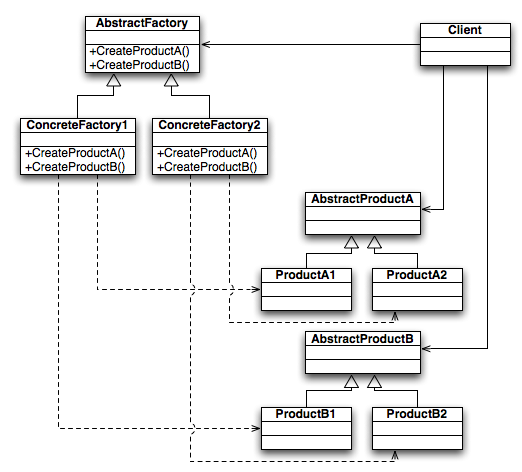
\includegraphics[scale=1]{../images/AbsFactory.png}
		\caption{Design Pattern Abstract Factory}
	\end{center}
	\end{figure}
	\begin{itemize}
		\item\textbf{Scopo}: fornire al Client un'interfaccia per creare famiglie di prodotti, senza dover esplicitare il nome concreto delle classi a cui si riferisce. La factory, quindi, incapsula le responsabilità per la creazione degli oggetti prodotto.
		\item\textbf{Applicabilità}:
		\begin{itemize}
			\item quando si necessita di rendere indipendente un sistema dalla creazione dei suoi componenti, dalla loro rappresentazione e composizione.
			\item quando si necessita la configurazione di un sistema scegliendo tra più tipologie.
			\item quando si devono gestire famiglie di prodotti correlati tra loro e progettati per essere usati insieme.
			\item quando si vuole rivelare solamente l'interfaccia delle classi all'interno di una libreria.
		\end{itemize}
		\item\textbf{Conseguenze}:
		\begin{itemize}
			\item isola le classi concrete, controllandone la creazione. La creazione è delegata
alla classe astratta e i Client manipolano solamente interfacce non conoscendo
i nomi dei prodotti nascosti
			\item permette di modificare facilmente la famiglia di prodotti utilizzati poiché la
classe concreta appare una sola volta nel programma
			\item promuove la coerenza nell'utilizzo dei prodotti poiché sono stati progettati per
essere utilizzati insieme (si usano oggetti di una sola famiglia per volta)
			\item risulta invece difficile l'inserimento di nuove tipologie di prodotto poichè richiederebbe la modifica della classe di Abstract Factory e di conseguentemente il
cambiamento di tutte le sottoclassi (il problema può essere evitato mediante
una tecnica di implementazione della classe astratta, ma in modo meno flessibile e poco sicuro.
		\end{itemize}
		\item\textbf{Utilizzo}: nel sistema Quizzipedia il design pattern è stato utilizzato nei package Interpreter e QuestionManager. Entrambi si avvalgono del pattern per rendere il sistema indipendente dalla creazione delle rispettive classi concrete e rendere i package aperti all'estensione tramite la definizione di nuovi tipi "Interpreter" e "Question".
	\begin{figure}[h!]
	\begin{center}
		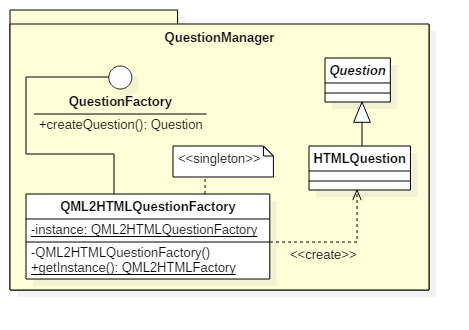
\includegraphics[scale=0.6]{../images/QuestionManagerClassDesignPattern.png}
		\caption{Abstract Factory in QuestionManager}
	\end{center}
	\end{figure}
	\begin{figure}[h!]
	\begin{center}
		\includegraphics[scale=0.5]{../images/interpreterClass.png}
		\caption{Abstract Factory in Interpreter}
	\end{center}
	\end{figure}
	\end{itemize}
	
	\subsection{Singleton}
	\begin{figure}[h!]
	\begin{center}
		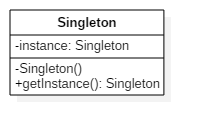
\includegraphics[scale=0.7]{../images/Singleton.png}
		\caption{Design Pattern Singleton}
	\end{center}
	\end{figure}
	\begin{itemize}
		\item\textbf{Scopo}: assicurare l'esistenza di una sola istanza di un oggetto, offrendo un punto globale di accesso a tale istanza.
		\item\textbf{Applicabilità}:
		\begin{itemize}
			\item quando deve essere creata una sola istanza di una classe e deve esistere un punto di accesso ad essa noto a tutti Client
			\item quando l'istanza deve poter essere estesa e i Client devono essere in grado di
utilizzarne le istanze senza apportare modifiche al proprio codice
		\end{itemize}
		\item\textbf{Conseguenze}:
		\begin{itemize}
			\item l'accesso all'unica istanza è controllato
			\item permette di aver un miglior uso delle variabili globali, riducendo lo spazio dei nomi senza inquinarlo con variabili utilizzate per memorizzare riferimenti ad
istanze
			\item maggior  flessibilità per quanto riguarda le operazioni di classe, ma maggior
difficoltà nelle modifiche del progetto per utilizzare più istanze. Impossibilità
di sovrascrivere le funzioni di classe poiché statiche e non virtuali.
		\end{itemize}
		\item\textbf{Utilizzo}: nel sistema Quizzipedia il design pattern è stato utilizzato per le classi\\
		 QML2HTMLQuestionFactory e QMLInterpreterFactory. Usato in collaborazione con\\ l'\emph{Abstract Factory}, il pattern assicura che la costruzione degli oggetti Interpreter e Question abbia un unico punto d'accesso nelle classi sopracitate.
	\end{itemize}
	\newpage
	
	\subsection{Builder}
	\begin{figure}[h!]
	\begin{center}
		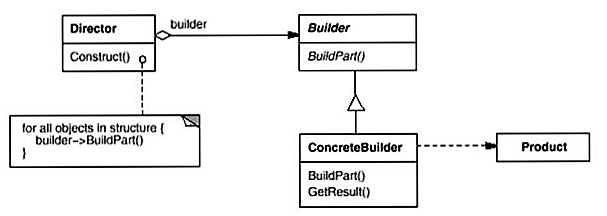
\includegraphics[scale=1]{../images/Builder.png}
		\caption{Design Pattern Builder}
	\end{center}
	\end{figure}
	\begin{itemize}
		\item\textbf{Scopo}: Separa la costruzione di un oggetto complesso dalla sua rappresentazione.
		\item\textbf{Applicabilità}:
		\begin{itemize}
			\item La procedura di creazione di un oggetto complesso
deve essere indipendente dalle parti che
compongono l'oggetto
			\item Il processo di costruzione deve permettere diverse
rappresentazioni per l'oggetto da costruire.
		\end{itemize}
		\item\textbf{Conseguenze}:
		\begin{itemize}
			\item Facilita le modifiche alla rappresentazione interna di
un prodotto
			\item Isola il codice dedicato alla costruzione di un prodotto
dalla sua rappresentazione
			\item Consente un controllo migliore del processo di
costruzione
		\end{itemize}
		\item\textbf{Utilizzo}: nel sistema Quizzipedia il design pattern è stato utilizzato nel package QuizManager per rendere la creazione di un Quiz indipendente dalle domande che lo compongono.
		\begin{figure}[h!]
	\begin{center}
		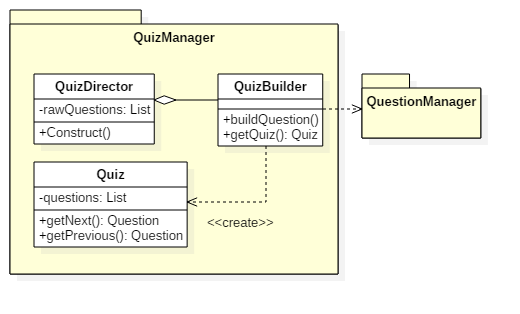
\includegraphics[scale=0.54]{../images/QuizManagerClass.png}
		\caption{Builder in QuizManager}
	\end{center}
	\end{figure}
	\end{itemize}
	\newpage
	
	\subsection{Command}
	\begin{figure}[h!]
	\begin{center}
		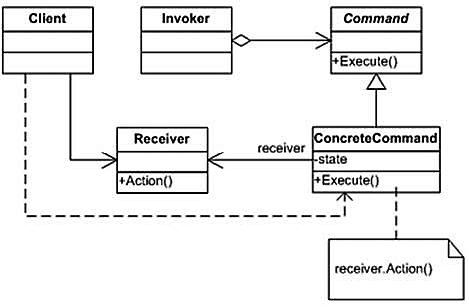
\includegraphics[scale=1]{../images/Command.png}
		\caption{Design Pattern Command}
	\end{center}
	\end{figure}
	\begin{itemize}
		\item\textbf{Scopo}: Incapsulare una richiesta in un oggetto, cosicché i
client sia indipendenti dalle richieste
		\item\textbf{Applicabilità}:
		\begin{itemize}
			\item Necessità di gestire richieste di cui non si conoscono i
particolari
			\item Parametrizzazione di oggetti sull'azione da eseguire
			\item Specificare, accodare ed eseguire richieste molteplici
volte
			\item Supporto ad operazioni di Undo e Redo e a transazioni.
		\end{itemize}
		\item\textbf{Conseguenze}:
		\begin{itemize}
			\item Accoppiamento "lasco" tra oggetto invocante e
quello che porta a termine l'operazione
			\item I command possono essere estesi
			\item I command possono essere composti e innestati
			\item È facile aggiungere nuovi comandi, le classi esistenti non devono essere modificate.
		\end{itemize}
		\item\textbf{Utilizzo}: nel sistema Quizzipedia il design pattern è stato utilizzato nel package Presenter, per disaccoppiare la ricezione degli input da parte della classe InputManager dalla loro risoluzione da parte di altre classi del Presenter e del Model. Il pattern permette inoltre di aggiungere facilmente nuovi \emph{Command} al sistema, estendendo l'interfaccia \emph{Input} del package UserInputManager. Sarà in questo modo più facile estendere le funzionalità offerte all'utente dal sistema Quizzipedia.
	\end{itemize}
	\begin{figure}[h!]
	\begin{center}
		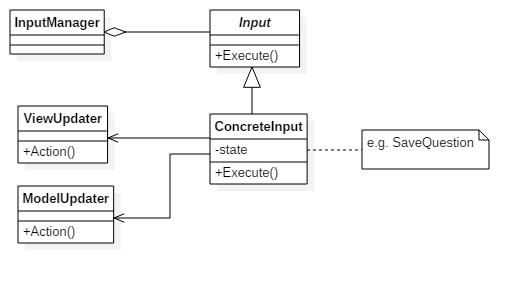
\includegraphics[scale=0.7]{../images/PresenterCommandDesignPattern.png}
		\caption{Design Pattern Command nel Presenter}
	\end{center}
	\end{figure}
	\newpage